\chapter{Kernel machines}
\label{cha:kernel_machines}

SVMs allow both linear and non linear problems. We saw a solution for non-linear SVMs that consists in a map in non-linear features as combination of features. This is a solution that is valid also for perceptrons. 
Therefore is not specific to SVMs but it becomes computationally unfeasible in high dimensional cases.
Also you need to find the correct map and it is a non trivial procedure.
The dual formulation of the SVMs (both classification and regression), the feature map only appear in dot products, which gets really expensive.\\

For SVMs we can do non-linear learning in a different way, this allows with infinite dimention spaces (the \textit{kernel} trick).\\

\defi{\textbf{Kernel trick}\label{def:kernel_trick}\\
The \textit{kernel trick} consists in replacing the dot products that appear in the dual formulation of non-linear SVMs with an equivalent kernel function:
$$k(\pmb{x}, \pmb{x'}) = \Phi(\pmb{x})^T \Phi(\pmb{x'})$$
The kernel function uses example in \textit{input space} (not feature). We can build a function that can compute this without to explicitly build the map.
}

As before, the dual optimization problem is 
$$max_{\alpha \in \R^m}\sum_{i=1}^m \alpha_i - 
    \frac{1}{2} \sum_{i} \sum_{j} \alpha_i y_i \alpha_j y_j \Phi(\pmb{x_i}) ^T \Phi(\pmb{x_j}) $$
in which $\Phi$ only appears as dot product.
subejct to:
$$\alpha_i \geq 0 \quad i = 1, \dots, m$$
$$\sum_{i=1}^m \alpha_i y_i = 0$$
The dual decision function is
$$f(\pmb{x}) = \sum _{i=1} ^m \alpha_i y_i \Phi(\pmb{x}_i)^T \Phi(\pmb{x'}) = \sum _{i=1} ^m \alpha_i y_i k(\pmb{x}_i , \pmb{x'})$$
in which $\Phi(\pmb{x}_i)^T \Phi(\pmb{x'})$ is in fact the dot product. I can replace the dot product with $k(\pmb{x}, \pmb{x'}) = \Phi(\pmb{x}_i)^T \Phi(\pmb{x'})$, since $\pmb{x}$ does not appear anywhere else, we are done.\\

\textbf{Kernelizing different SVMs}\\
This procedures also works for different types of SVMs, therefore we can make appear $\Phi$ only in dot products. In Figure \ref{fig:SVM_regression_kernel} an example for regression.\\
\begin{figure}[ht]
    \centering
    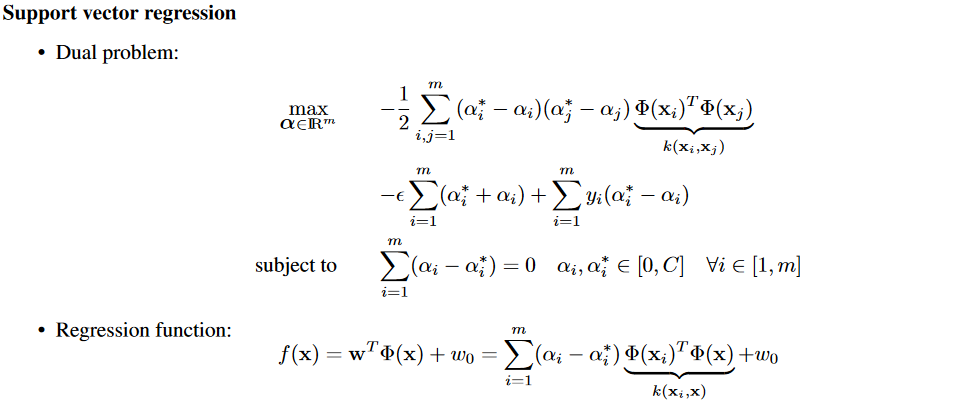
\includegraphics[scale=0.5]{images/kernel_SVM_regression.png}
    \caption{Procedure applied for SVM used in a regression case}
    \label{fig:SVM_regression_kernel}
\end{figure}

\textbf{Kernelizing a perceptron}\\
The kernel procedure can be also be applied on perceptrons: a linear function of a perceptron \textit{kernelized} becomes a non-linear function.\\
We can take the dual formulation of the perceptron. Remember that in kernel machines (in both regression and classification), $f(x)$ is a combination of the sum over the train examples coefficient times the kernel function.
For a classic stochastic perceptron, the procedure is the following: at first we set 
$$\pmb{w} = 0$$
then we iterate until all examples are correctly classified (stochastic perceptron) and we update each incorrectly classified examples: 
$$\pmb{w} \leftarrow \pmb{w} + \eta y_i \pmb{x}_i$$
We learn this coefficient going through the data. \\

For a kernel perceptron it becomes: 
at first we initialize
$$\alpha_i = 0 \quad \forall i$$
then we iterate through the examples and for each miss-classified example we perform an update:
$$\alpha_i \leftarrow \alpha_i + \eta y_i$$
The kernel perceptron classification function becomes
$$f(\pmb{x}) = \sum _{i=1} ^m \alpha_i k(\pmb{x}_i, \pmb{x})$$


\section{What are kernels}
    Let's see and example of a polynomial mapping (both homogeneous and inhomoeneous). 
    \begin{figure} [ht]
        \centering
        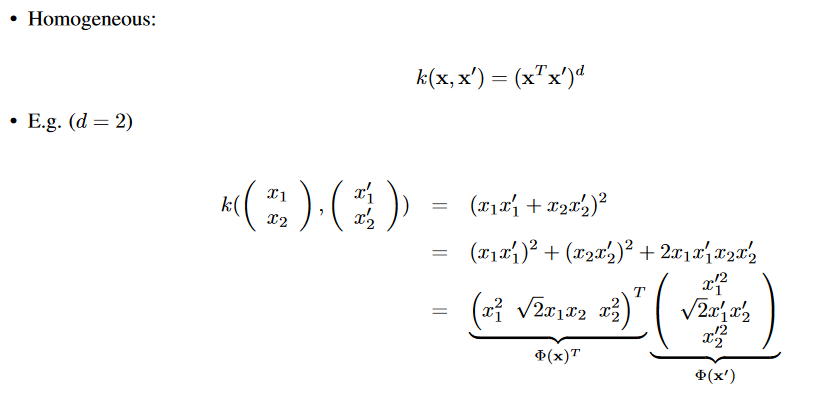
\includegraphics[scale=0.5]{images/homo_poly.png}
        \caption{Example of homogeneous polynomial kernel}
        \label{fig:homo_poly_kernel}
    \end{figure}
    We can substitute the $k(\pmb{x}, \pmb{x}')$ with $(\pmb{x}^T, \pmb{x}')^d$ (dot product in input space) at the power of $d$, whose result is a scalar. The number of operations depends on the number of input features, not on the size of the features space.\\
    \textbf{A kernel it always correspond to a dot product in some feature space.}
    For each piece of the sum of the second line, we need to to separate $\pmb{x}$ from $\pmb{x}'$. 
    Therefore, in this case the dot product corresponds to $\Phi(\pmb{x})^T \Phi(\pmb{x}')$, which makes it a dot product (polynomial mapping, aside from the coefficient). 
    We did not explicitely compute $\Phi$ but we computed only at input-space level.\\
    In this case we compute two summation instead of three, bit with greater feature spaces and powers then we get a large advantage.
    We are computing a polynomial mapping in a non-explicit way.\\

    It is also more effective in the case of an inhomogeneous polynomial kernel, in which not only we have combination of degree $d$ but also all combination with degree\textit{ up to} d $\leq d$. This increases a lot the number of features. 
    We can compute it by summing $1$ to the dot product in input space before raising to the power of $d$. Adding $1$ corresponds to a dot product in a inhomogeneous polynomial mapping. The procedure is similar.
    Again, we separate $\pmb{x}$ from $\pmb{x}'$ and we get two $\Phi$ functions, which contain term with degree up to $d$. Also in this case we did explicitly computed in feature-space level.
    \begin{figure}[ht]
        \centering
        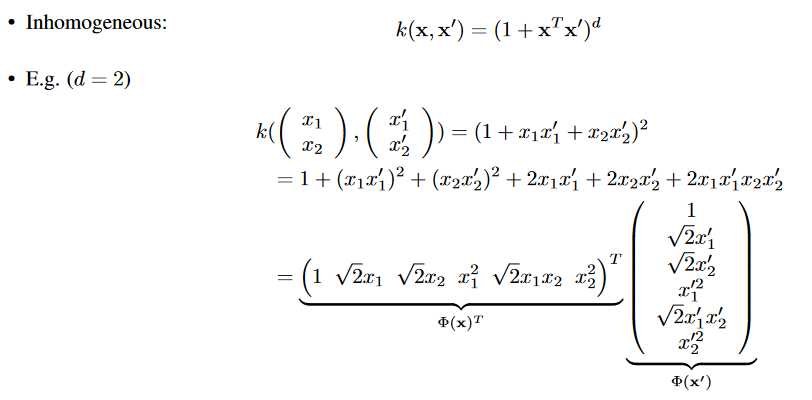
\includegraphics[scale=0.5]{images/inho_kernel.png}
        \caption{Example of inhomogeneous polynomial kernel}
        \label{fig:inhomo_poly_kernel}
    \end{figure}

    The fact that we rise in an $\R ^n$ dimensional space does not change complexity since we are raising scalars. Usual we do not use high complexity spaces because we would get too many features and we risk overfitting.\\

    This is possible only because we are working in the \textit{dual form} and we get $\pmb{x}$ only as dot products.

    \defi{\textbf{Kernel}\label{def:kernel}\\
    A valid \textbf{kernel} what works properly, is a function defined over the cartesian product of the input space
    $$k: \mathcal{X} \times \mathcal{X} \rightarrow \R $$
    that correspond to a dot product in \textit{some} feature space
    $$k(\pmb{x}, \pmb{x}')= \Phi(\pmb{x})^T \Phi(\pmb{x}')$$
    Kernels can be seen as similarities between objects.  
    }
    Indeed, you can apply kernels to input that are not vectors at all (as sequences or graphs). We can define kernels on arbitrary structures. 
    In practice, we can apply several algorithms to these object via this kernel that implicitly maps these object in some vectors.

\section{Validity of a kernel}
    In many cases, if we build learning systems on non-vector object we have to invent the kernel ourselves, therefore we need to verify that it is a valid one. 
    
    \defi{\textbf{Gram matrix}\label{def:gram_matrix}\\
    Given examples $\{\pmb{x}_1, \dots, \pmb{x}_m\}$ and a kernel function $k$, the \textit{Gram matrix K} is the symmetric matrix pf pairwise kernels between examples:
    $$K_{ij} = k(\pmb{x}_i, \pmb{x}_j) \quad \forall i, j$$ 
    This matrix is symmetric. 
    }
    
    \defi{\textbf{Positive definite matrix}\label{def:pos_def_matrix}\\
    A symmetric $m \times m$ matrix $K$ is a positive (\textit{semi-})definite if
    $$\sum_{i, j = 1} ^m \pmb{c}_i \pmb{c}_j K_{ij} \geq 0 \quad \forall \pmb{c} \in \R^m$$
    If equality only holds for $\pmb{c} = 0$, the matrix is \textit{strictly positive definite}.
    All eigenvalues of $K$ are non negative, or are positive (for strictly positive definite). 
    }
    
    It is not enough to see what happens only on the training set matrix: we would like to show that the \textit{function} is positive definite, that it is indeed a function.
    There is a direct way to do it which is an eigen-decomposition for functions, which will not be discussed and could be tricky.\\
    
    The easier way to show this validity is checking the satisfaction of at least one of these conditions and requisites:
    \begin{itemize}
        \item prove its positive definiteness (difficult)
        \item find corresponding feature map: explication of $\Phi$ dot-product combination by making the feature map explicit
        \item use kernel combination properties in order to build a new kernel, the operation that we can perform on kernels will preserve their properties.
    \end{itemize}

\section{Types of kernels}
    Two principal types of kernels are 
    \begin{itemize}
        \item linear $$k(\pmb{x}, \pmb{x}') = \pmb{x}^T \pmb{x}'$$
        \item polynomial, that can be parameterized 
        $$k_{c, d} (\pmb{x}, \pmb{x}') = (\pmb{x}^T \pmb{x}' + c) ^d$$
        \item Gaussian kernel \ref{cha:gaussian_kernel}
    \end{itemize}

    \subsection{Gaussian kernel}
        \label{cha:gaussian_kernel}
        Apart from the coefficients typical of the normal, it is the same as a Gaussian distribution.  
        We can assume that one of the two input is the sample and the other the mean (the Gaussian is symmetric, so it does not matter the order).
        \begin{align*}
            k_{\sigma} (\pmb{x}, \pmb{x}') &= exp {\left(- \frac{||\pmb{x} - \pmb{x}'||^2}{2 \sigma^2} \right) } \\
                &= exp {\left( - \frac{\pmb{x}^T \pmb{x} - 2 \pmb{x}^T \pmb{x}' + \pmb{x}'^T\pmb{x}' }{2\sigma^2} \right)}
        \end{align*}
        This is an exponential detection of the difference between the values. This is an exponentially decaying kernel.\\
        
        First: if we unroll the square norm, we get a Gaussian kernel that can be computed as dot products in input space, and then we operate scalar operation that produce a Gaussian kernel.
        Once again, the complexity is bounded to the input space.\\
        A Gaussian kernel has an infinite dimension feature space, this determines a useful property called \textit{universality}: this means that it can uniformly approximate any function (provided it is continuous). 
        In principle, with a Gaussian kernel, we can approximate any (continuous) function.\\

        The problem of this kernel is finding the correct value of $\sigma$, the larger the value, the more tolerance we allow (on the other hand: the higher, the stricter, then only the closest training sample will impact the prediction, more similar to kNN). 

    \subsection{How to choose}
        The choice of the kernel (also the choice of $\sigma$ for a Gaussian kernel) has to be made before the training, so we need to specify them in term of cross-validation.

\section{Kernels on structured data}
    We previously said that kernel machines come with the nice feature of the possibility of being applied on data structures different than vectors. 
    By working in the dual we can replace $\pmb{x}$ with the kernel function, I can apply the learning algorithm and I am sure to compute large margin solution in feature space, even if the input space is a non-vector space.
    In this case, the kernel can be seen as a way of generalizing the dot product in arbitrary spaces. 
    This is the driving principle of designing a kernel.\\

    A kernel of a structure is typically built in terms of \textit{combination of kernels over pieces} (structures have lot of pieces, and then combined). Here some types of kernels on structures ($x$ are not vectors anymore)
    \begin{itemize}
        \item \textbf{match kernel} (or \textit{delta}) which consists in a delta function: 
        \begin{equation}
          k_{\sigma} (x, x') = \delta(x, x') =\left\{
          \begin{array}{@{}ll@{}}
            0, & \text{if}\ x=x' \\
            1, & \text{otherwise}
          \end{array}\right.
        \end{equation} 
        This does not make sense with vectors (low generalization). It makes sense indeed when we use this in combination.
        \item \textbf{string kernel 3-gram spectrum kernel} which basically looks at frequencies.
        \begin{figure}[ht]
            \centering
            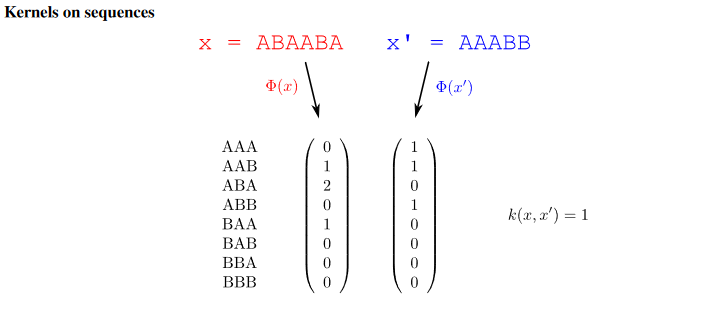
\includegraphics[scale=0.5]{images/string_kernel.png}
            \caption{example of kernel applied on sequences}
            \label{fig:string_kernel}
        \end{figure}
        It looks at how many times the triplet appears as continuous sub-sequences in $x$ and compare them with same sub-sequences in $x'$. Then the kernel does a dot-product in this feature space. 
    \end{itemize}

    \subsection{Building kernel as combination}
        Build a kernel by combining pieces means build a valid kernel by following some rules that ensure validity. 
        \begin{enumerate}
            \item simpler kernel can be combined using certain operation ($+, \times, \dots$) 
            \item Kernel combination allows to design complex kernels on structures from simpler ones
            \item correctly using combination operators guarantees that complex kernels are preserved
        \end{enumerate}

        \subsubsection{Kernel summation}
            The sum of two kernels corresponds to the \textit{concatenation} of their respective feature space.
            \begin{figure}[ht]
                \centering
                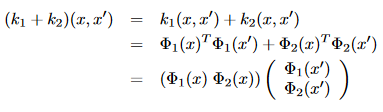
\includegraphics[scale=0.7]{images/kernel_sum.png}
                \caption{Summation of two kernels}
                \label{fig:kernel_sum}
            \end{figure}
            The assumption is of course the combination of valid kernels. 
            $k_1, k_2$ could look at different part of the input, not necessarily the same (example two different portion or characteristic of strings).

        \subsubsection{Kernel multiplication}
            The product of valid kernel is a valid kernel. 
            \begin{figure}[ht]
                \centering
                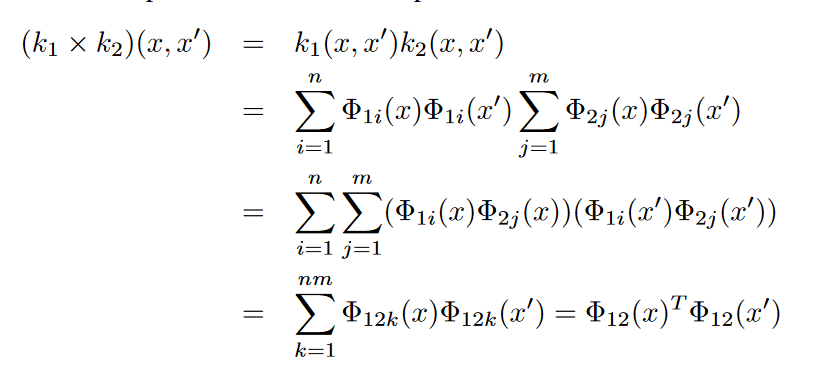
\includegraphics[scale=0.4]{images/kernel_mul.png}
                \caption{Multiplication of two kernels}
                \label{fig:kernel_mul}
            \end{figure}
            where $\Phi_{12}(x) = \Phi_1 (x) \times \Phi_2 (x)$ is the cartesian product between the spaces of the two kernels.
            We have to compute over every combination of features. The feature space that comes out of it is more complex. This already explodes the feature spaces. \\
            Still, this is a valid combination. 

        \subsubsection{Liner combination}
            We can always multiply a kernel by a scalar, provided that the scalar is non-negative (would invert every prediction). We can define a kernel as linear combination of kernels. 
    		$$k_{sum}(x, x') = \sum_{k=1}^K\beta_k k_k(x,x')$$
            Since understanding which kernel to use for a specific problem is non trivial, we can use a linear combination of different kernels and then learn parameters of kernels $\beta$ along with learning $\alpha$. 
            We can learn both coefficient jointly to select which kernel is more useful (\textbf{kernel learning}). 

        \subsubsection{Decomposition kernels}
            We need to decompose our structure in some way we can apply different kernels. 
            We can do it hierarchically, another way to formalizing the decomposition is using a \textbf{decomposition kernel} or \textbf{convolutional} kernels. 
            This works by having a \textit{decomposition relationship} that takes one object and brakes it into \textit{parts} 
            $$R(x)= (x_1, x_2, \dots, x_D)$$
            A decomposition kernel is 
            $$(k_1 * \dots * k_D)(x, x') = 
                \sum _{(x_1, \dots, x_D) \in R(x)} \sum _{(x'_1, \dots, x'_D) \in R(x')} 
                \prod_{d=1} ^ D k_d(x_d, x'_d) $$
            We compute a kernel, we sum over every possible decomposition of the two objects according to their decomposition function and then we compare the two decomposition (in the convolution case) as the products of the single pieces. 
            $k_d$ is a kernel on pieces that could be hierarchically defined (or simply the match kernel).\\ 

            \textbf{Set kernel}\\
            This is a very simple example, basically the decomposition relationship is the set - membership. Therefore the overall kernel is the sum of overall combinations of the kernel between them. 
            $$k_{set} (X, X') = \sum _{\xi \in X} \sum _{\xi' \in X'} k_{member} (\xi, \xi')$$
            This becomes easy when the $k_{member}$ function is a delta function. 

        \subsubsection{Kernel normalization}
            When working with structures, a problem could be that you use different dimensional objects (the similarity of a ling sequence will be higher than the one computed on a short sequence). 
            Therefore we need to normalize our kernels by taking into account the size of the structure
            $$\hat{k}(x,x') = \frac{k(x,x')}{\sqrt{k(x,x)k(x',x')}}$$
            At the denominator we get exactly the norm. 
            This particular normalization is the \textit{cosin normalization} because it takes into account the angle between the two (we are getting rid of th esize of the object). 

        \subsubsection{Kernel composition}
            We can build not only by combining, but also via composition. Instead of having $x^T x$ in the Gaussian kernel, we can plug another kernel and put is as input of the Gaussian kernel. 
            
    		$$(k_{d,c}\circ k)(x,x') = (k(x,x')+c)^d$$
    		$$(k_\sigma\circ k)(x,x') = exp\left({-\frac{k(x,x)-2k(x,x')+k(x',x')}{2\sigma^2}}\right)$$

            This gets us to a composition of kernels. This project us in higher dimensional space. 

    \subsection{Kernel on graphs (WL kernel)}
        We can also exploit kernel on structured data as graphs. The Weistfeiler-Lehman (WL) graph kernel relies in the WL approximation for graphs isomorphism. This is an efficient way of dealing with kernel on graphs.

        \subsubsection{WL isomorphism test}
            This test is conducted on two graphs $\mathcal{G} = \{E, V\}, \mathcal{G'} = \{E', V'\}$ with equal number of vertices. 
            Let $\mathcal{L}(\mathcal{G})$ a label function for each node in $\mathcal{G}$ such that contains $l(v)$ for each node $ v \in V $. There is also a label function for $\mathcal{G}'$ and they need to contain the same labels. 
            The algorithm goes like this:
            \begin{enumerate}
                \item set $l_0 (v) = l(v)$ for all v (set initial labels of the graph $\mathcal{G}$ as the given labels for that graph).
                \item for each $i \in [ 1 \dots |V| ]$
                \begin{enumerate}
                    \item for each node $v$ in $\mathcal{G}, \mathcal{G'}$
                    \begin{enumerate}
                        \item construct a list of sorted labels $M_i (v)$ of the adjacent nodes of $v$ of the previous step
                        $$M_i (v) = \{ l_{i-1} (u) \} \qquad \forall u \text{ adjacent to } v$$
                        \item concatenate the label for the node $v$ at previous step with the $m_i (v)$ list (Figure \ref{fig:WL_iso_1}), also use a function $label$ that assigns unique labels to the string (Figure \ref{fig:WL_iso_2}) (could be for example an hash function)
                        $$l_i (v) = label (l_{i-1} (v), M_i(v))$$
                    \end{enumerate}
                    \item if $l_i(\mathcal{G}) \neq l_i(\mathcal{G'})$
                    \begin{enumerate}
                        \item \textbf{return FALSE}   
                    \end{enumerate}
                \end{enumerate}
                \item \textbf{return TRUE}
            \end{enumerate}

            \begin{figure}[ht]
                \centering
                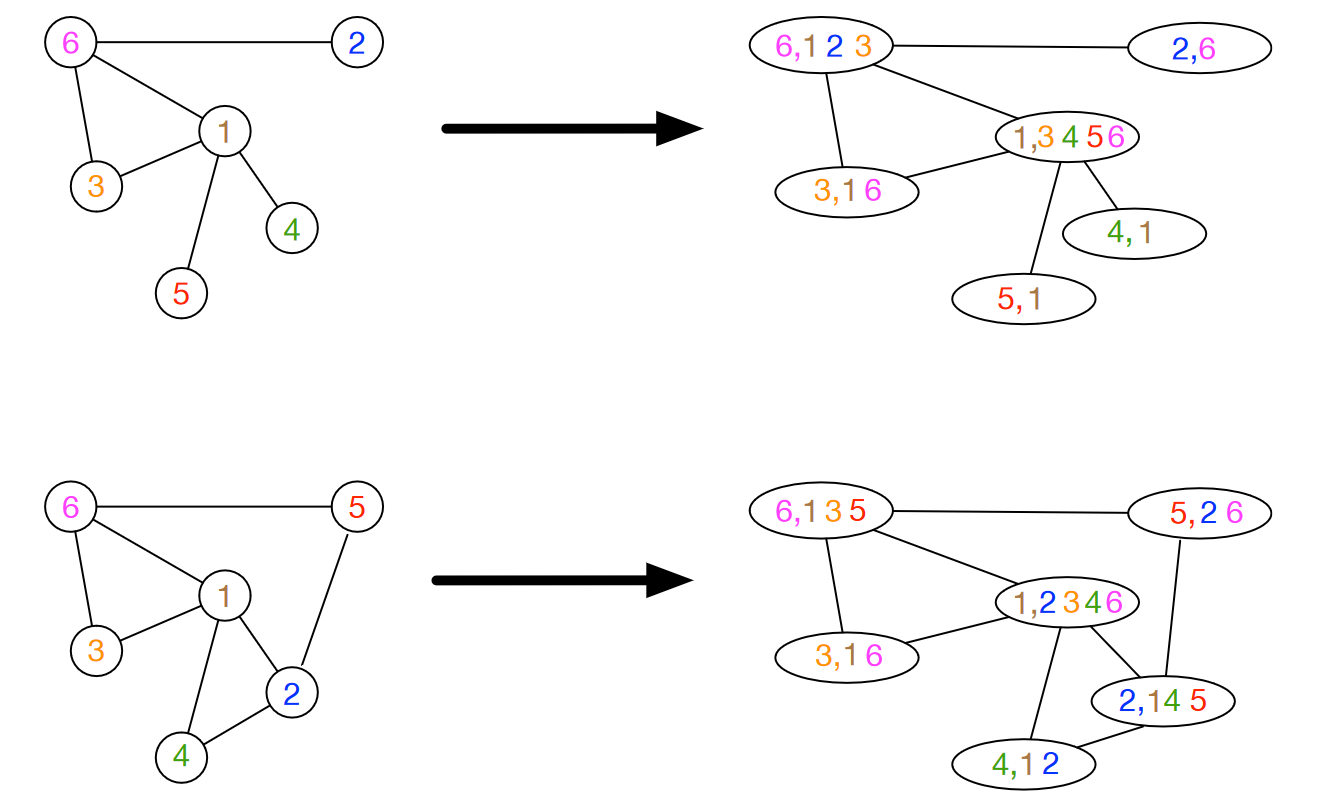
\includegraphics[scale=0.3]{images/graph_labeling.png}
                \caption{WL-isomorphism test, we are assigning to each node a string that contains the labels of all adjacent nodes}
                \label{fig:WL_iso_1}
            \end{figure}

            \begin{figure}[ht]
                \centering
                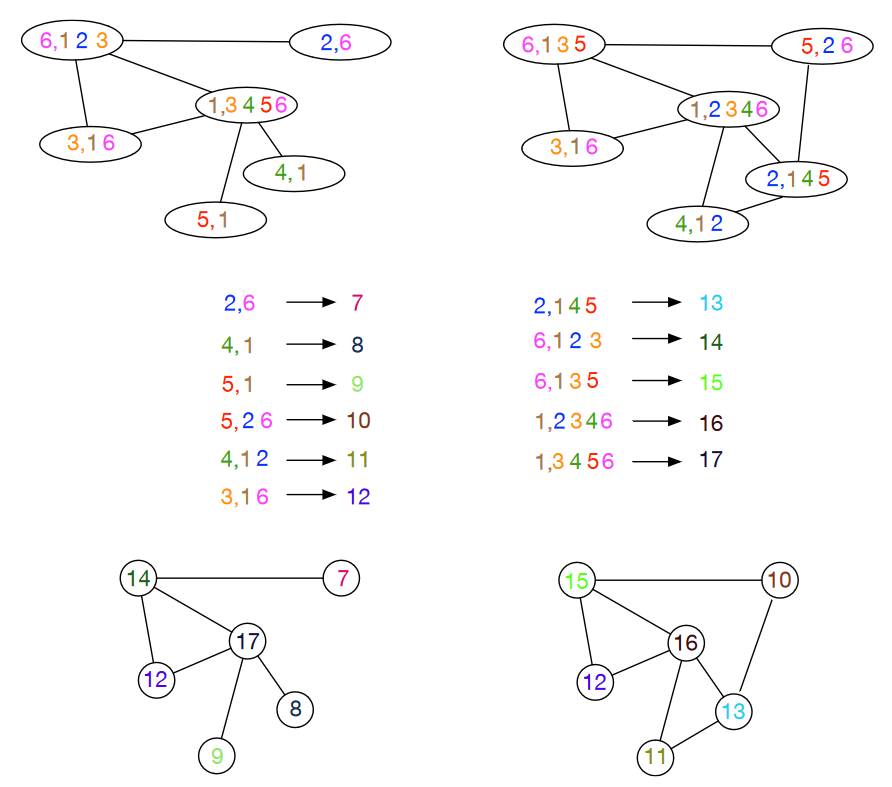
\includegraphics[scale=0.4]{images/graph_re_labeling.png}
                \caption{WL-isomorphism test, we using the $label$ function to convert the string into unique labels}
                \label{fig:WL_iso_2}
            \end{figure}

        \subsubsection{WL graph kernel}
            Let $\{\mathcal{G}_0, \dots, \mathcal{G}_h \} = \{ (V, E, l_0), \dots, (V, E, l_h) \}$ a sequence of graphs made from $\mathbf{G}$, where we are identifying the label $i$ as the \textit{i-th} iteration of the WL algorithm.
            Let $k : \mathcal{G} \times \mathcal{G}' \rightarrow \R$ any kernel on graph. Then the WL graph kernel is defined as 
            $$k_{WL} ^ h (\mathcal{G}, \mathcal{G}') = \sum _{i=0} ^ h k(\mathcal{G}_i, \mathcal{G}_i ')$$

            \begin{figure}[ht]
                \centering
                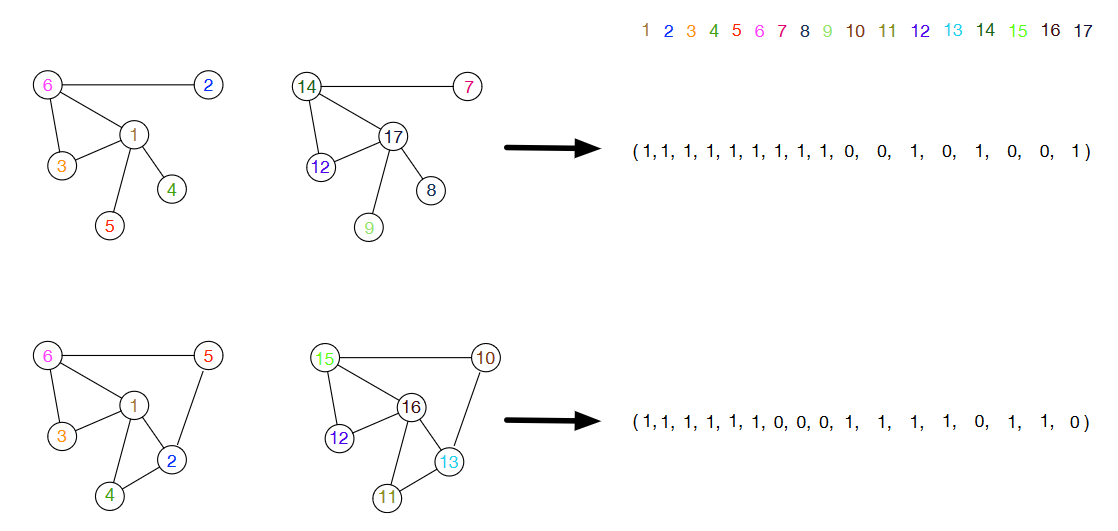
\includegraphics[scale=0.5]{images/graph_kernel.png}
                \caption{Execution of the graph kernel. This kernel will use a string in which it will store 1 or 0 respectively if it has found the i-th label in the graph or not. }
                \label{fig:ML_kernel}
            \end{figure}
            